\chapter{Single-Lepton Stop Search}
\label{chap:stop}

This chapter will describe a search for supersymmetry with the target signal
being stop-antistop squark pairs decaying to a single-lepton (1$\ell$)
final state. This work was performed using the CMS experiment during
Run II of the LHC, at 13 TeV center-of-mass energy. This analysis
resulted in two publications: the search performed using 2016 data \cite{stop1l},
and a combined single-lepton and all-hadronic search using 2015 data
\cite{combination0l}. Two public research documents (PASes) were
also produced to support conference results \cite{pasichep,pasmoriond},
however these are superceded by the published results. I will focus on
the analysis as described in Reference \cite{stop1l}, particularly my work
developing the compressed T2tt search strategy.

\section{Motivation}
\label{sec:stop:motivation}

As Section \ref{ssec:susy:rationale} has described, supersymmetry
(SUSY) is a very important class of theories in particle physics. It
has the potential to solve the hierarchy problem, and may provide the
answer to the difficult question of what particles make up dark
matter. And the notion of naturalness would seem to imply that our
current or near-future particle colliders have just the right energies
to search for evidence of SUSY.

One particularly interesting feature of SUSY is that if you arrange
the sparticles in order from lightest to heaviest, they will generally line up
in reverse order from the Standard Model particles. So whereas the
electron is the lightest stable SM particle, and the top quark is the
heaviest, by contrast the stop squark is expected to be one of the lightest
sparticles, and the selectron one of the heaviest. We say SUSY has an
\emph{inverted mass hierarchy}. % Cite this!
% See refs 8-12 in 8 TeV stop paper.
This means that the Lightest Supersymmetric Particle ($\lsp$), the
chargino ($\chargino$), and the stop squark ($\tilde{t}$) should be
some of the easiest sparticles to detect.
% The single-lepton channel provides a nice balance between
% cross-section and ease of ID.

\section{Previous Searches}
\label{sec:stop:run1}

A search for stop pairs in the one-lepton final state was previously
performed at CMS during Run I \cite{stop1l8tev}. This search used 19.5
fb$^{-1}$ of 8 TeV collision data. The analyzers performed a traditional
cut-based search, and also a search employing a boosted decision tree
(BDT). This machine-learning technique allows a computer to attempt to
discriminate between signal and background. Ultimately, neither search
strategy detected any evidence of the production of stop squarks. This
result allowed the analyzers to set limits on the possible masses of
stops and LSPs. Specifically, stop squarks were excluded up to masses
of about 650 GeV in the case where the LSP is massless, and LSPs were
excluded up to a maximum of 200-250 GeV for stop masses around 500-600
GeV.

The LHC and the CMS detector received a number of upgrades for Run II,
some of which have greatly benefitted the single-lepton stop
search. Of particular note, the LHC collision energy was raised from 8
to 13 TeV, which increases the likelihood of producing heavy new
particles, and the luminosity was increased considerably, allowing us % Quantify lumi increase
to record more data in the same amount of running time. In addition,
we have learned from the Run I analysis, and attempted to improve our
analysis techniques for Run II. To avoid the obfuscation inherent in
results produced by machine learning, we declined to perform a BDT
search. We also added a new signal model to our search. Finally, we
added dedicated signal regions to address the unique kinematics of
several particular regions of phase space.

% How about any ATLAS stop-1L searches?
% Or searches from CDF or D0?
% It's hard, because there are a LOT of searches that set limits on
% stops in general.

\section{Signal Models}
\label{sec:stop:sigmodels}

Because supersymmetry is still a theoretical construct, and the masses
of the sparticles are unknown, there are a number of possible
ways that a stop squark pair could decay to a single lepton final
state. We consider three possible signal models, each with its own
unique signature. In addition, we consider a wide range of possible
masses for our sparticles, and the kinematics that result.

\subsection{Bulk Signals}
\label{ssec:stop:sigbulk}

\subsubsection*{T2tt}

One of the primary models we target is known by the identifer
\textbf{T2tt}. In this model, the stop squarks decay to top quarks and
LSPs ($\tilde{t} \rightarrow t \lsp_1$). The top quarks then decay to
bottoms and W bosons, as normal; one of the Ws decays leptonically,
and the other hadronically. The two free parameters in this model are
the stop mass, $\mstop$, and the LSP mass, $m_{\lsp_0}$; we
scan a wide range of possible values for these two variables. The
kinematics of the decay products are determined entirely by the stop
and LSP masses. A diagram of the T2tt model is pictured at the top of
Figure \ref{fig:stop:feynmandiagrams}.

\subsubsection*{T2bW}

The second primary model we consider is known as \textbf{T2bW}. In this
model, the stop squarks decay to bottom quarks and charginos, skipping
the top quarks entirely. The charginos then decay to W bosons and
neutralinos ($\tilde{t} \rightarrow b \chargino_1, \chargino_1 \rightarrow
W \lsp_1$). One W then decays leptonically, and the other
hadronically. In this case, the free parameters are $\mstop$,
$m_{\lsp_0}$, and also the chargino mass, $\mchargino$. For the
purposes of this analysis, we fix the chargino mass at the average of
the stop and neutralino masses, $\mchargino = (\mstop
+ \mlsp) / 2$. We then scan a broad range of possible values
for $\mstop$ and $\mlsp$. We also created a set of
dedicated signal regions targeting the case where $\mchargino$ and
$\mlsp$ are nearly identical. The T2bW model is diagrammed in
the middle of Figure \ref{fig:stop:feynmandiagrams}.

\subsubsection*{T2tb}

For the Run II search, we have added a new signal model that was not
evaluated in the Run I search. This model is called \textbf{T2tb}. It
is essentially a mixture of the T2tt and T2bW models, in that it
covers the case where one of the stop squarks decays to a top quark
and an LSP, and the other decays to a bottom quark and a chargino. For
this analysis, we fix $\mchargino$ to be $\mlsp + 5$ GeV. We
then scan a range of possible values for $\mstop$ and
$\mlsp$. The T2tb model is pictured at the bottom of Figure
\ref{fig:stop:feynmandiagrams}.

% Insert Feynman diagrams. Either make them, or pull from the documentation.

\subsection{Compressed T2tt}
\label{ssec:stop:sigcompressed}

There is a region of the $\mstop$ and $\mlsp$ phase space
that is of particular interest to us in this analysis. In the T2tt
model, if the difference between the stop and LSP masses is less than
the mass of the top quark, $\mstop - \mlsp \lesssim m_t$, then the top quark
must be produced off-shell (i.e. with a mass that is not its normal
$\sim$173 GeV). This kind of process would be difficult to detect
because the production of off-shell top quarks is suppressed, and
because there is also less energy and momentum available to the top
deca products. We may also consider what happens if we go one step
further, to the region where $\mstop - \mlsp \lesssim m_W$. In this case, not
only the top quark but also its resultant W boson must be produced
off-shell, making it even harder to detect this signal. We call these
cases ``compressed'' T2tt decays, because the phase space available to
the decay products is squeezed down to a smalle range.

The difficulties in detecting compressed T2tt signals are evident in
the results plot of the Run I analysis \cite{stop1l8tev}. The exclusion
curve for the T2tt model has no coverage in the narrow strip where
$\mstop - \mlsp \approx m_t$, or the strip where $\mstop - \mlsp
\approx m_W$. We call these two regions the \emph{top corridor} and
the \emph{W corridor}, respectively. In this analysis we wished to
fill in these two gaps, and achieve exclusion in the corridor
regions. To that end, I developed a specialized set of
signal regions that target the kinematics of compressed decays, with
the aim of increasing our sensitivity to these signals. These
specialized signal regions will be described in Section
\ref{ssec:stop:corridorsrs}, and the compressed T2tt search will be
described separately from the nominal search in cases where
the two strategies differ.

\section{Datasets and Triggers}
\label{sec:stop:datatrig}

\subsection{Data samples}
\label{ssec:stop:datasamples}

There are two main signatures that we use to search for our stop
decays. The first is the presence of a single, isolated lepton. This
signature is fairly obvious, because we chose to search in the single
lepton final state. In addition, all of our signal models have two
LSPs and a neutrino in the final state. The LSPs should go undetected
by the CMS detector, just as neutrinos do, so we also expect our
signals to appear with large amounts of MET.

With these two main signatures in mind, we select our data from the
Single Lepton and MET datasets produced by the CMS
experiment. We also employ the single muon or electron dataset for certain control
regions to be described in Section \ref{ssec:stop:lostlep}, and the
single photon datasets for MET resolution studies to be % Need reference to MET resolution studies
described in Section \ref{}. These datasets were recorded during the
2016 datataking period, encompassing eras 2016B through 2016H, and
represent a total integrated luminosity of 35.9 fb$^{-1}$. Table
\ref{tab:stop:datasets} gives a complete listing of all datasets used
in the analysis.

% Homemade table of datasets goes here. %%%%%%%%%%%%%% Would be nice to add run ranges!
\begin{table}[htbp]
\centering
\caption{List of datasets used in the analysis.}
\label{tab:stop:datasets}
\begin{tabular}{l}
\hline
Dataset \\
\hline
  /SingleMuon/Run2016B-03Feb2017\_ver2-v2/MINIAOD \\
  /SingleMuon/Run2016C-03Feb2017-v1/MINIAOD \\
  /SingleMuon/Run2016D-03Feb2017-v1/MINIAOD \\
  /SingleMuon/Run2016E-03Feb2017-v1/MINIAOD \\
  /SingleMuon/Run2016F-03Feb2017-v1/MINIAOD \\
  /SingleMuon/Run2016G-03Feb2017-v1/MINIAOD \\
  /SingleMuon/Run2016H-03Feb2017\_ver2-v1/MINIAOD \\
  /SingleMuon/Run2016H-03Feb2017\_ver3-v1/MINIAOD \\
\hline
  /SingleElectron/Run2016B-03Feb2017\_ver2-v2/MINIAOD \\
  /SingleElectron/Run2016C-03Feb2017-v1/MINIAOD \\
  /SingleElectron/Run2016D-03Feb2017-v1/MINIAOD \\
  /SingleElectron/Run2016E-03Feb2017-v1/MINIAOD \\
  /SingleElectron/Run2016F-03Feb2017-v1/MINIAOD \\
  /SingleElectron/Run2016G-03Feb2017-v1/MINIAOD \\
  /SingleElectron/Run2016H-03Feb2017\_ver2-v1/MINIAOD \\
  /SingleElectron/Run2016H-03Feb2017\_ver3-v1/MINIAOD \\
\hline
  /MET/Run2016B-03Feb2017\_ver2-v2/MINIAOD \\
  /MET/Run2016C-03Feb2017-v1/MINIAOD \\
  /MET/Run2016D-03Feb2017-v1/MINIAOD \\
  /MET/Run2016E-03Feb2017-v1/MINIAOD \\
  /MET/Run2016F-03Feb2017-v1/MINIAOD \\
  /MET/Run2016G-03Feb2017-v1/MINIAOD \\
  /MET/Run2016H-03Feb2017\_ver2-v1/MINIAOD \\
  /MET/Run2016H-03Feb2017\_ver3-v1/MINIAOD \\
\hline
  /MuonEG/Run2016B-03Feb2017\_ver2-v2/MINIAOD \\
  /MuonEG/Run2016C-03Feb2017-v1/MINIAOD \\
  /MuonEG/Run2016D-03Feb2017-v1/MINIAOD \\
  /MuonEG/Run2016E-03Feb2017-v1/MINIAOD \\
  /MuonEG/Run2016F-03Feb2017-v1/MINIAOD \\
  /MuonEG/Run2016G-03Feb2017-v1/MINIAOD \\
  /MuonEG/Run2016H-03Feb2017\_ver2-v1/MINIAOD \\
  /MuonEG/Run2016H-03Feb2017\_ver3-v1/MINIAOD \\
\hline
  /SinglePhoton/Run2016B-03Feb2017\_ver2-v2/MINIAOD \\
  /SinglePhoton/Run2016C-03Feb2017-v1/MINIAOD \\
  /SinglePhoton/Run2016D-03Feb2017-v1/MINIAOD \\
  /SinglePhoton/Run2016E-03Feb2017-v1/MINIAOD \\
  /SinglePhoton/Run2016F-03Feb2017-v1/MINIAOD \\
  /SinglePhoton/Run2016G-03Feb2017-v1/MINIAOD \\
  /SinglePhoton/Run2016H-03Feb2017\_ver2-v1/MINIAOD \\
  /SinglePhoton/Run2016H-03Feb2017\_ver3-v1/MINIAOD \\
\hline
\end{tabular}
\end{table}

\subsection{Triggers}
\label{ssec:stop:triggers}

For each of the datasets described above, we select events using
appropriate HLT triggers. Of particular note, we select data events
for our signal regions using the union of the single lepton and MET
triggers. This strategy allows us to use leptons that are below their
trigger thresholds, and to compensate for any inefficiency in the
turn-on phase of the MET trigger. The triggers we use are
listed in Table \ref{tab:stop:trigs}.

% Table of HLT triggers paths, adapted from AN-14-463, with a few modifications
\begin{table}[htb]
\caption{HLT trigger paths corresponding to each of the primary
  datasets used in the analysis. The trigger version is suppressed.}
\label{tab:stop:trigs}
\centering
\footnotesize
\begin{tabular}{|l|l|}
\hline
Type & HLT path \\
\hline
SingleMuon & HLT\_Iso(Tk)Mu22 OR HLT\_Iso(Tk)Mu24 \\
SingleElectron & HLT\_Ele25\_eta2p1\_WPTight\_Gsf OR HLT\_Ele27\_eta2p1\_WPTight\_Gsf \\
\hline
\multirow{3}{*}{MET} & HLT\_PFMET170\_HBHECleaned OR \\
 & HLT\_PFMET(NoMu)110\_PFMHT110(NoMu)\_IDTight OR \\
 & HLT\_PFMET(NoMu)120\_PFMHT120(NoMu)\_IDTight \\
\hline
\hline
\multirow{2}{*}{MuonEG} & HLT\_Mu8\_TrkIsoVVL\_Ele23\_CaloIdL\_TrackIdL\_IsoVL(\_DZ) OR \\ 
 & HLT\_Mu23\_TrkIsoVVL\_Ele12\_CaloIdL\_TrackIdL\_IsoVL(\_DZ) \\
\hline
\multirow{2}{*}{SinglePhoton} & HLT\_Photon*\_R9Id90\_HE10\_IsoM OR HLT\_Photon165\_HE10 OR \\
 & HLT\_Photon175 OR HLT\_Photon250\_NoHE \\
\hline
\end{tabular}
\end{table}

\subsection{Trigger efficiency measurements}
\label{ssec:stop:trigeff}

% It kinda helps to know what the lost lepton background is before
% this section
We measure the efficiency of our combined single lepton and MET
triggers in a sample of events from the JetHT primary dataset,
selected using the \verb+HLT_(PF)HT*+ trigger paths. We use events
triggered on $H_T$ because this trigger is expected to be orthogonal
to the MET and lepton $p_T$ triggers, allowing us to examine the full % Should I actually say how the efficiency is computed?
spectrum of these variables. The trigger
efficiency is parameterized in MET and lepton $p_T$. We select events
with at least one lepton and two jets. Our definitions of leptons,
jets, and MET are presented later, in Section
\ref{sec:stop:selections}.

Figure \ref{fig:stop:trigeff:1lepmet} shows the parameterized trigger
efficiencies, separated by flavor of the leading lepton. Using 35.9 fb$^{-1}$
of data, our overall trigger efficiency is 99.1\% in the region MET $>$
250 GeV and lepton $p_T >$ 20 GeV. Because this efficiency is so close
to 100\%, we do not correct for the small inefficiency. However, we
assign a systematic uncertainty of 2\% for events with MET below 300
GeV, and 4\% for events with MET greater than 300 GeV.

% Plots of trigger efficiency taken from AN-16-463. Unpublished!
\begin{figure}[htb]
\centering
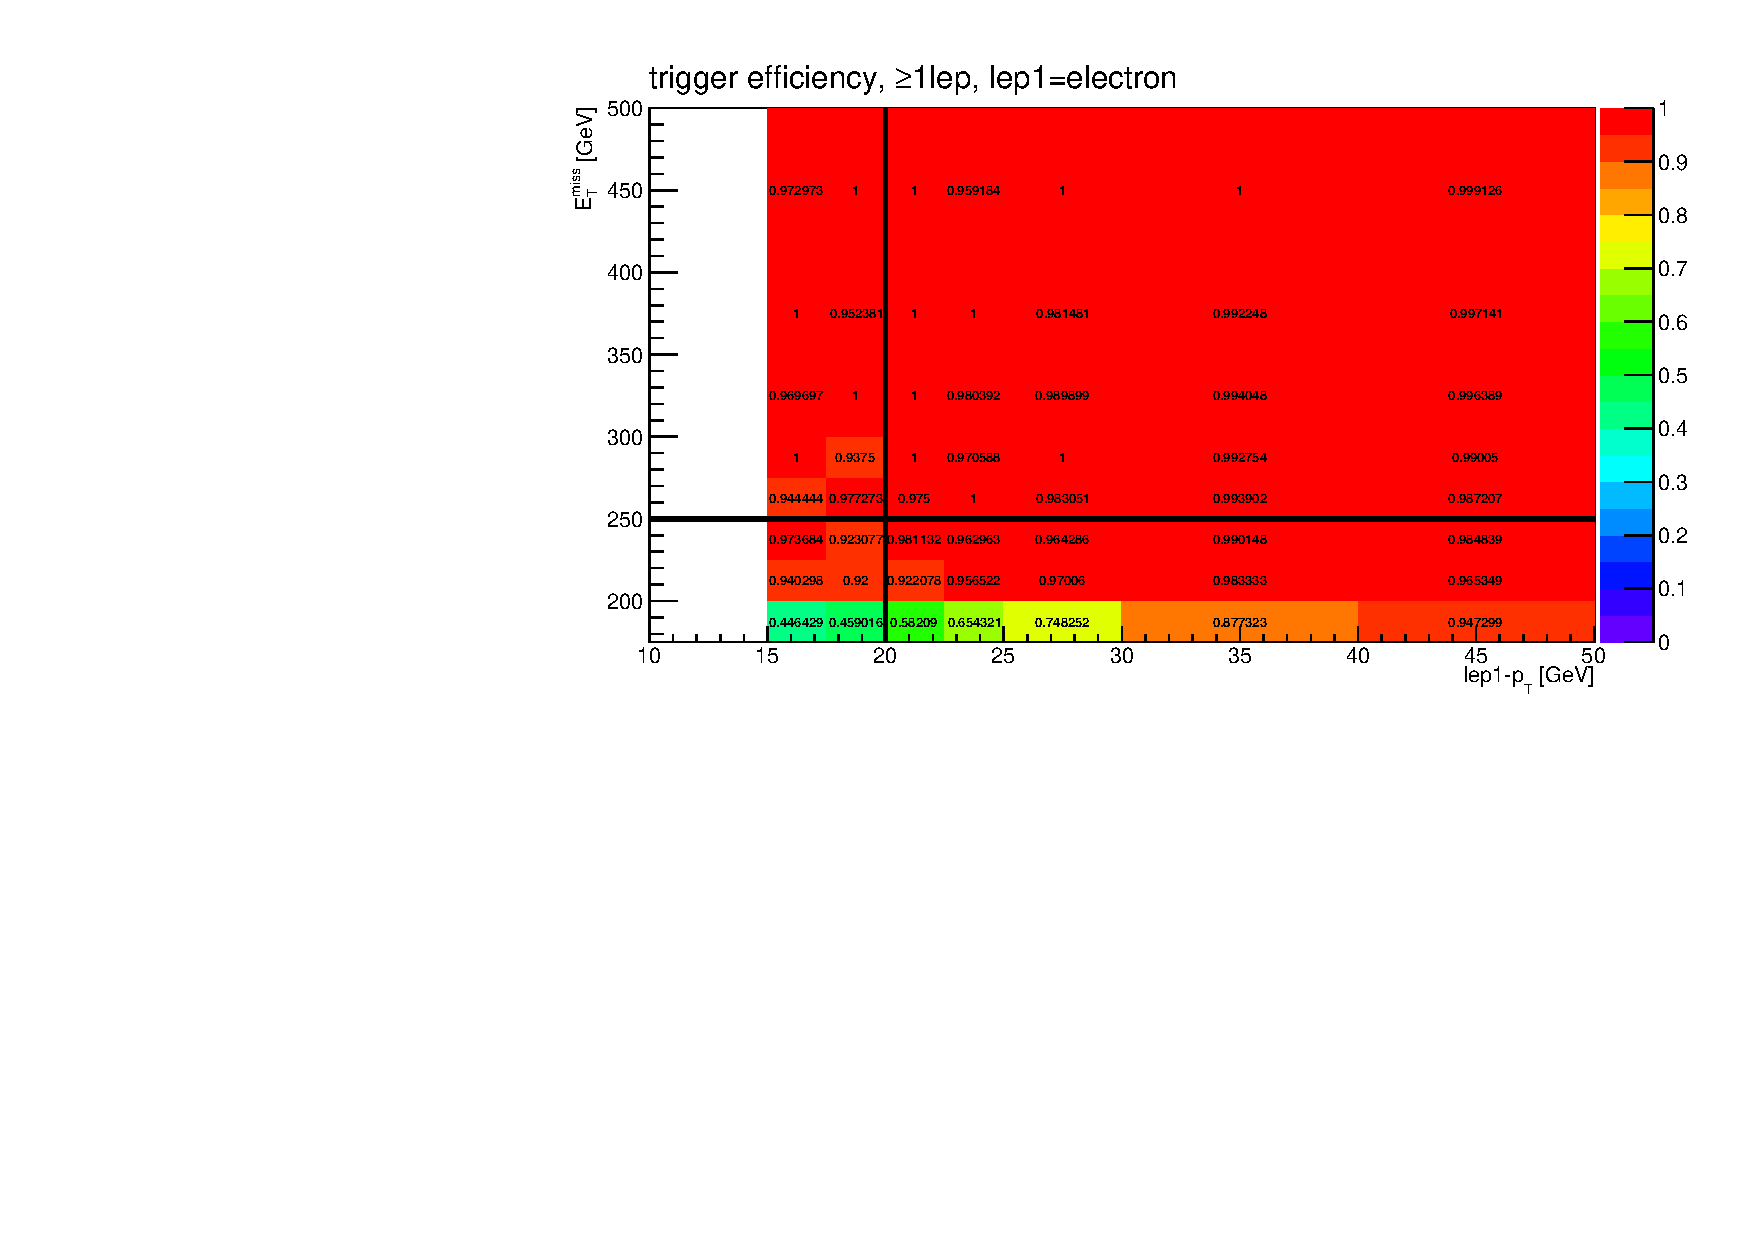
\includegraphics[width=0.45\textwidth]{figures/TriggerEff_el.pdf}
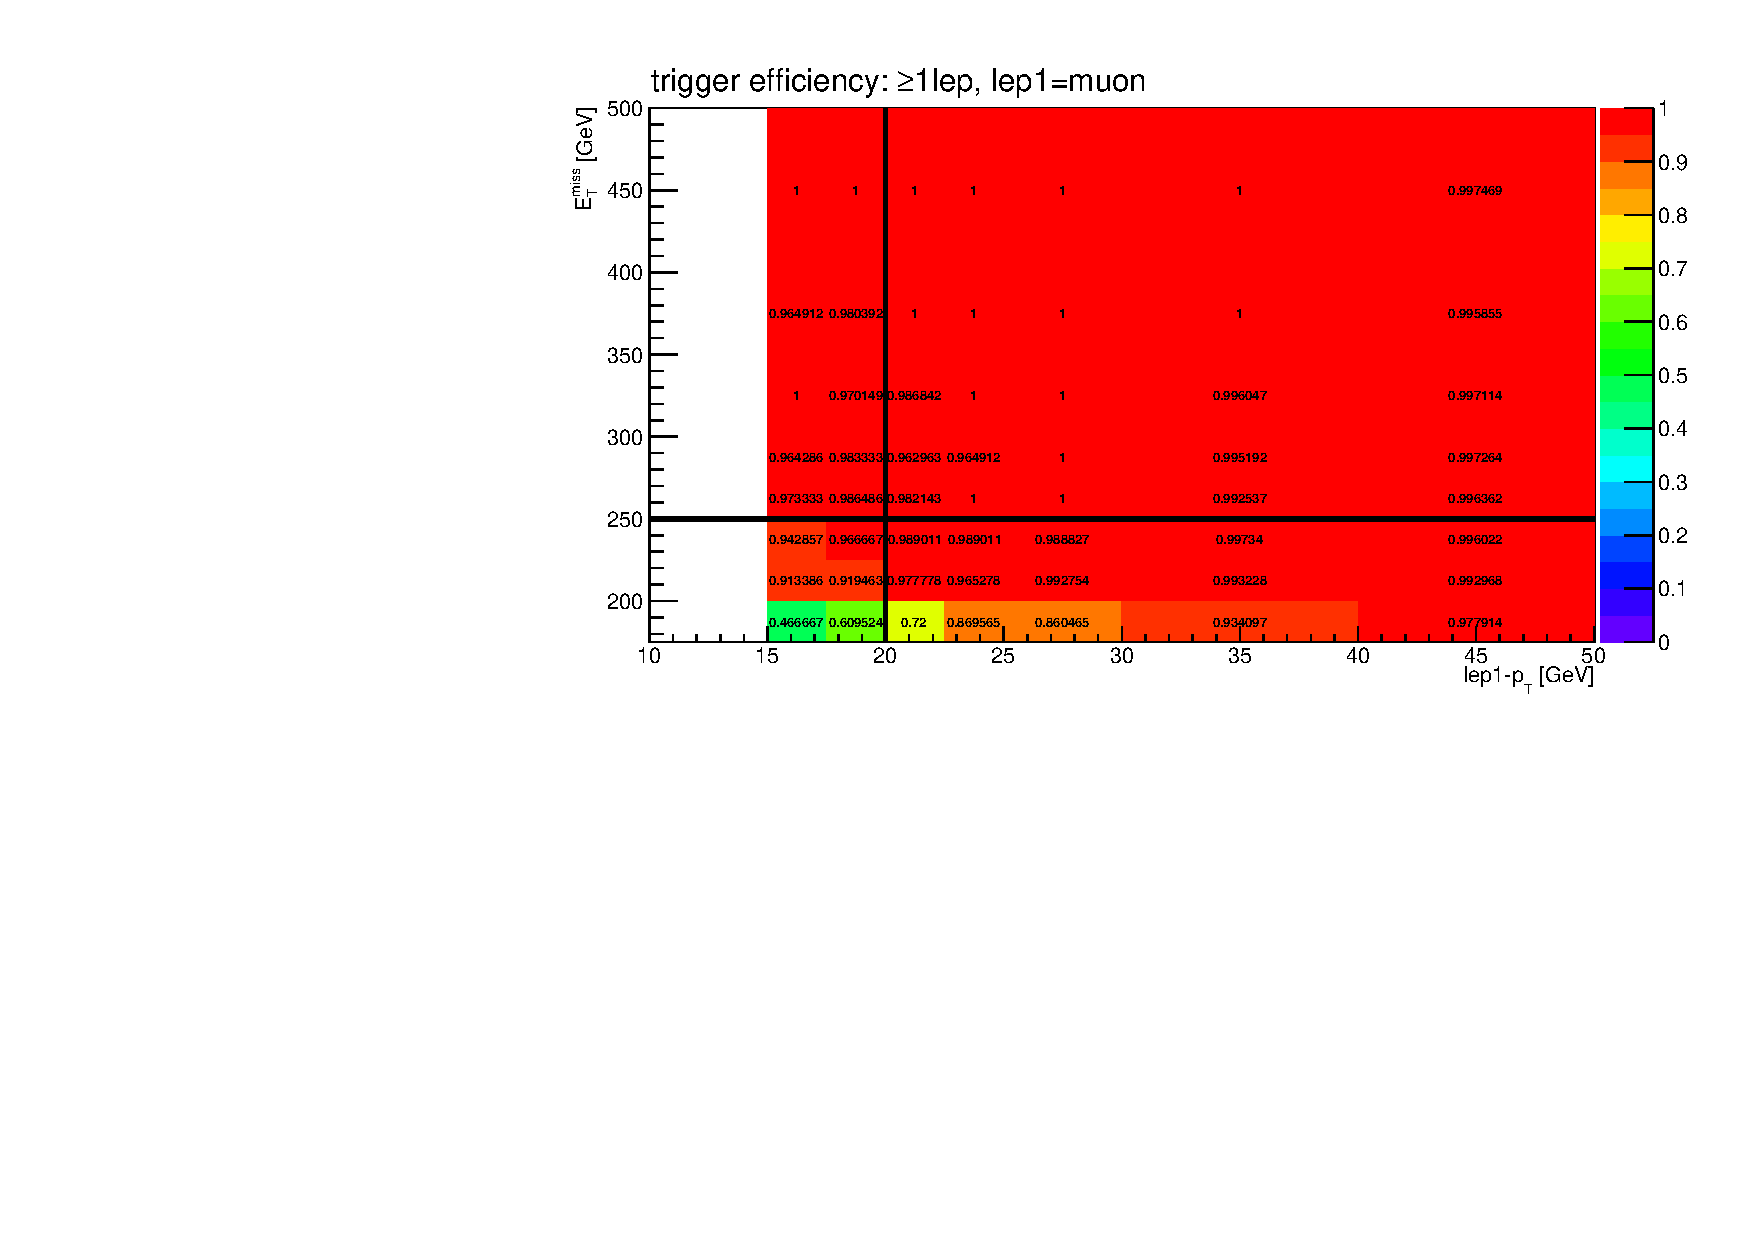
\includegraphics[width=0.45\textwidth]{figures/TriggerEff_mu.pdf}
\caption{Measured efficiencies for the union of the single lepton and
  MET triggers. Efficiency is represented by the z-axis color scale. The
  efficiencies are presented separately for the case where the leading
  lepton is an electron (left), and a muon (right).}
\label{fig:stop:trigeff:1lepmet}
\end{figure}

As Section \ref{ssec:stop:lostlep} will describe, certain of our
background estimation techniques compel us to treat the $p_T$ of a
second lepton as part of the MET. For this special case, we must
re-evaluate the efficiency of our combined single lepton and MET
triggers. We do so using the exact same procedures described above,
except that we additionally require events to have a second lepton
with $p_T >$ 10 GeV. These efficiencies are presented in Figure
\ref{fig:stop:trigeff:2ndlepplusmet}. Because the combined triggers
have substantial inefficiency at low MET and low lepton $p_T$, we
do correct our Monte Carlo simulations for these trigger
efficiencies when performing this background estimation.

% Plots of 2nd-lep-plus-met trigger efficiency taken from AN-16-463. Unpublished!
\begin{figure}[htb]
\centering
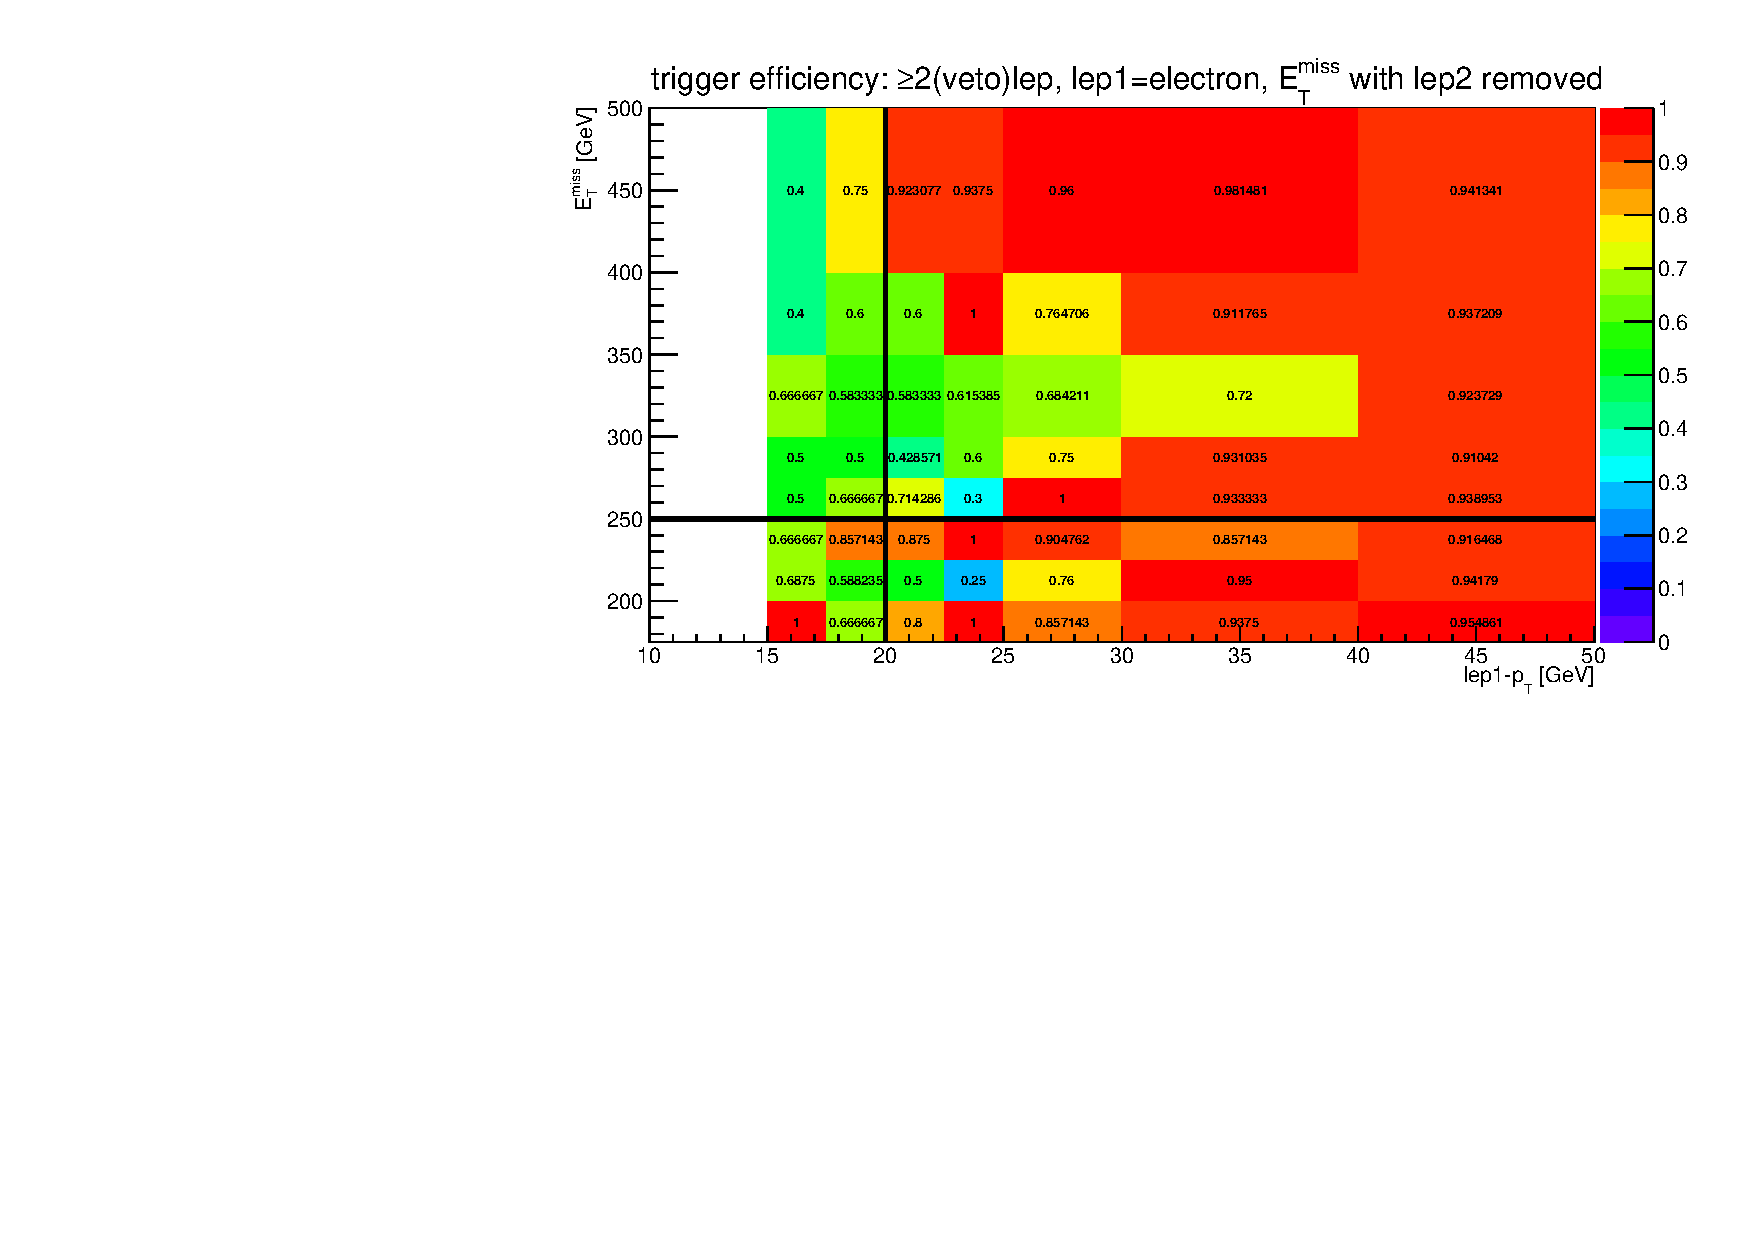
\includegraphics[width=0.45\textwidth]{figures/TriggerEff2l_el.pdf}
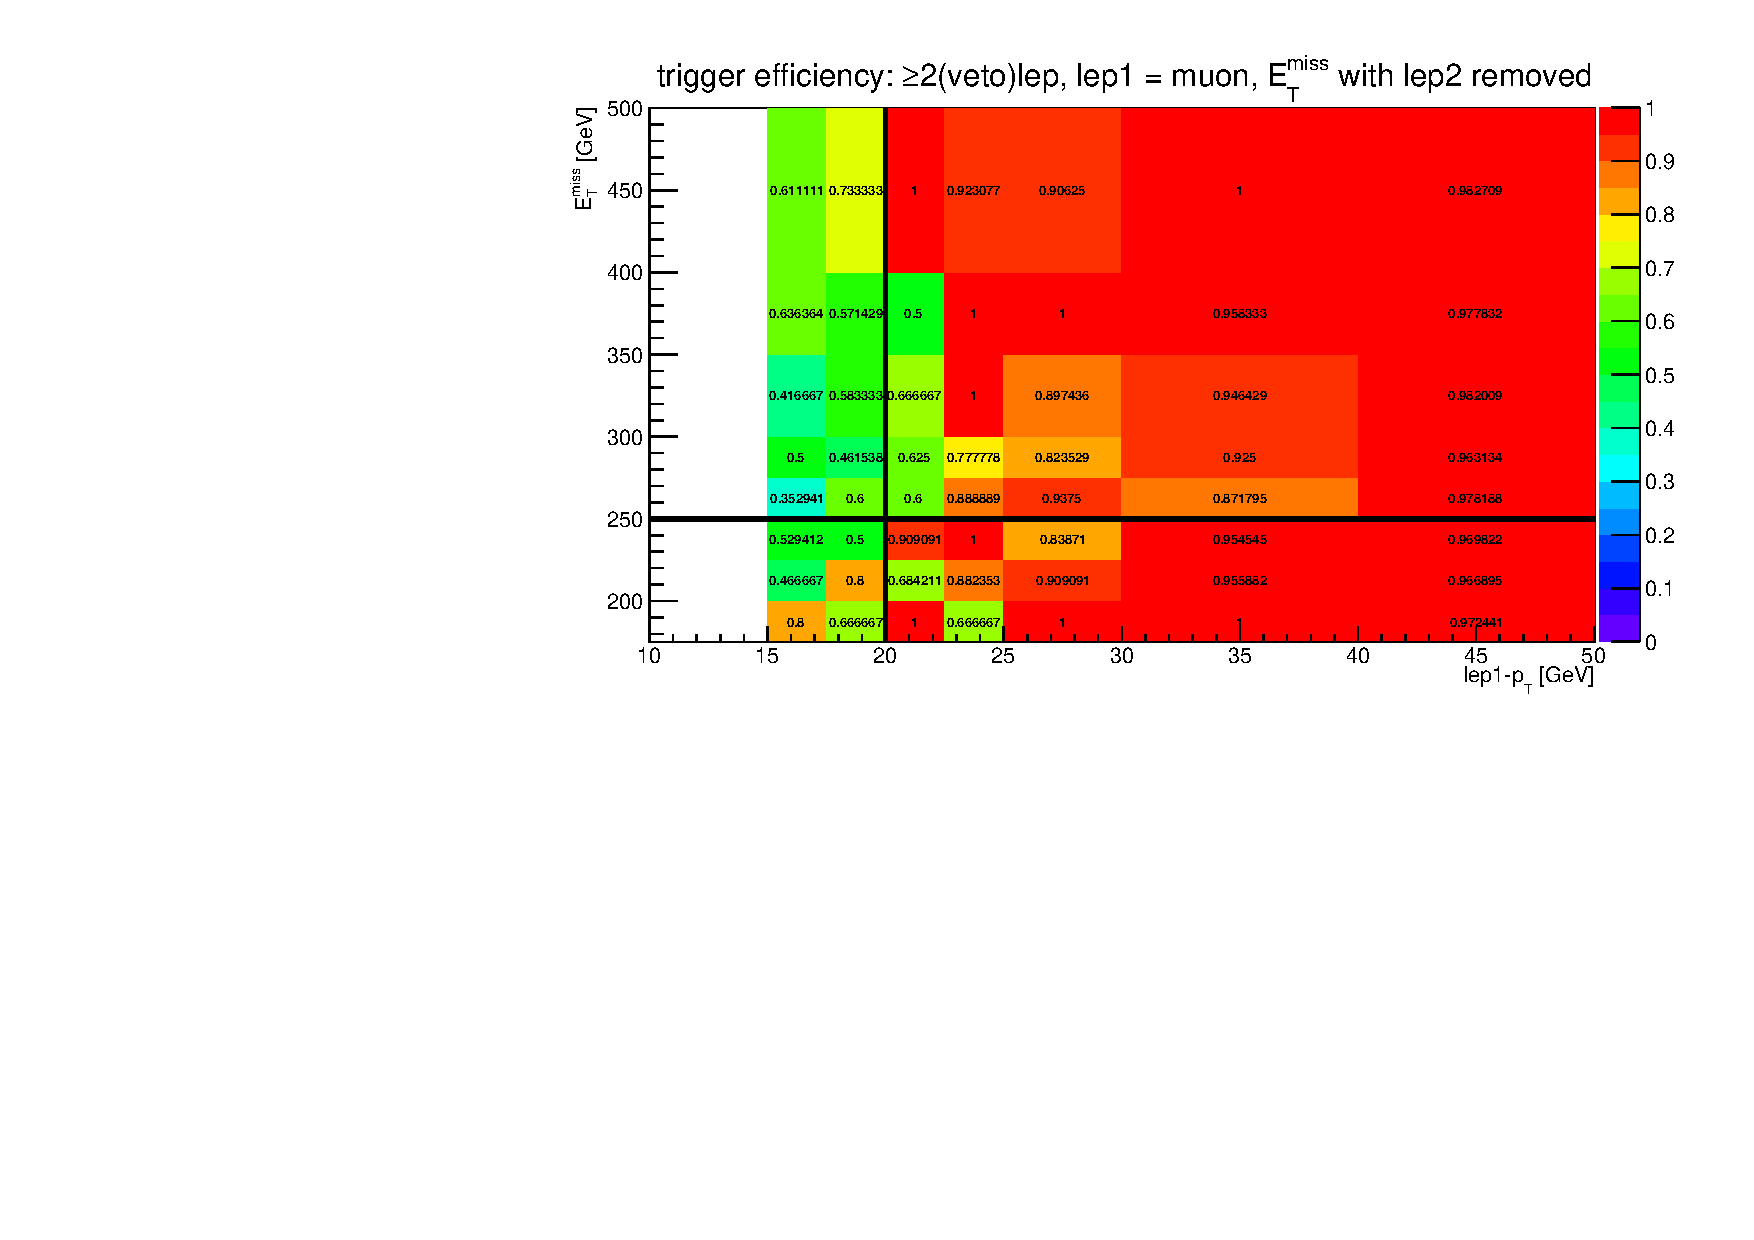
\includegraphics[width=0.45\textwidth]{figures/TriggerEff2l_mu.pdf}
\caption{Measured efficiencies for the union of the single lepton and
  MET triggers, when the subleading lepton $p_T$ is added to the
  MET. Efficiency is represented by the z-axis color scale. The
  efficiencies are presented separately for the case where
  the leading lepton is an electron (left), and a muon (right).}
\label{fig:stop:trigeff:2ndlepplusmet}
\end{figure}

% What to say about the dilepton and single photon trigger
% efficiencies? How are these evaluated? Do we present measured
% efficiencies anywhere?

\subsection{Monte Carlo samples}
\label{ssec:stop:mcsamples}

Our analysis relies on modeling a number of background and signal
processes using Monte Carlo simulation. Table \ref{tab:stop:mcsamples}
presents the complete list of Monte Carlo samples used. All samples
are produced as MINIAODSIM.

% Table of MC samples taken from AN-16-463. Unpublished.
\begin{table}[htp]
\caption{
  Monte Carlo simulation datasets used in this analysis, and their
  theoretical cross sections. The symbol * replaces the string
  RunIISummer16MiniAODv2-PUMoriond17\_80X\_mcRun2\_asymptotic\_2016\_TrancheIV\_v6, % Warning: underfull hboxes abound here!
  and the $\dagger$ replaces
  RunIISpring16MiniAODv2-PUSpring16Fast\_80X\_mcRun2\_asymptotic\_2016\_miniAODv2\_v0.}
\label{tab:stop:mcsamples}
\centering
%\makebox[\textwidth][c]{%
{\footnotesize
\begin{tabular}{|l|c|c|c|}
\hline
Sample & Cross Section \\
& [pb] \\
\hline
/TTJets\_SingleLeptFromT\_TuneCUETP8M1\_13TeV-madgraphMLM-pythia8/*(\_ext)-v1 & 182.7 \\
/TTJets\_SingleLeptFromTbar\_TuneCUETP8M1\_13TeV-madgraphMLM-pythia8/*(\_ext)-v1 & 182.7 \\
/TTJets\_DiLept\_TuneCUETP8M1\_13TeV-madgraphMLM-pythia8/*\_ext-v1 (and *-v4) & 87.3 \\
/ST\_tW\_top\_5f\_NoFullyHadronicDecays\_13TeV-powheg\_TuneCUETP8M1/*-v1 & 19.6 \\
/ST\_tW\_antitop\_5f\_NoFullyHadronicDecays\_13TeV-powheg\_TuneCUETP8M1/*-v1 & 19.6 \\
/ST\_t-channel\_top\_4f\_leptonDecays\_13TeV-powheg-pythia8\_TuneCUETP8M1/*-v1 & 44.1 \\ 
/ST\_t-channel\_antitop\_4f\_leptonDecays\_13TeV-powheg-pythia8\_TuneCUETP8M1/*-v1 & 26.2 \\
/ST\_s-channel\_4f\_leptonDecays\_13TeV-amcatnlo-pythia8\_TuneCUETP8M1/*-v1 & 3.7 \\
/W1JetsToLNu\_TuneCUETP8M1\_13TeV-madgraphMLM-pythia8/*-v1 & 11782  \\
/W2JetsToLNu\_TuneCUETP8M1\_13TeV-madgraphMLM-pythia8/*-v1 & 3841 \\
/W3JetsToLNu\_TuneCUETP8M1\_13TeV-madgraphMLM-pythia8/*-v1 & 1160 \\
/W4JetsToLNu\_TuneCUETP8M1\_13TeV-madgraphMLM-pythia8/*-v1 & 600 \\
/W1JetsToLNu\_NuPt-200\_TuneCUETP8M1\_13TeV-madgraphMLM-pythia8/*-v1 & 2.36  \\
/W2JetsToLNu\_NuPt-200\_TuneCUETP8M1\_13TeV-madgraphMLM-pythia8/*-v1 & 4.95 \\
/W3JetsToLNu\_NuPt-200\_TuneCUETP8M1\_13TeV-madgraphMLM-pythia8/*-v1 & 4.94 \\
/W4JetsToLNu\_NuPt-200\_TuneCUETP8M1\_13TeV-madgraphMLM-pythia8/*-v1 & 8.83 \\
/ttWJets\_13TeV\_madgraphMLM/*-v1 & 0.61 \\
/ttZJets\_13TeV\_madgraphMLM/*-v1 & 0.78 \\
/WWTo2L2Nu\_13TeV-powheg/*-v1 & 12.18 \\
/WWToLNuQQ\_13TeV-powheg/*-v1 & 50.00  \\
/WZTo3LNu\_TuneCUETP8M1\_13TeV-powheg-pythia8/*-v1 & 4.43 \\
/WZTo2L2Q\_13TeV\_amcatnloFXFX\_madspin\_pythia8/*-v1 & 5.60 \\
/WZTo1L1Nu2Q\_13TeV\_amcatnloFXFX\_madspin\_pythia8/*-v1 & 10.74 \\
/WZTo1L3Nu\_13TeV\_amcatnloFXFX\_madspin\_pythia8/*-v1 & 3.05 \\
/ZZTo4L\_13TeV\_powheg\_pythia8/*-v1 & 1.25 \\
/ZZTo2L2Q\_13TeV\_amcatnloFXFX\_madspin\_pythia8/*-v1 & 3.22 \\
/ZZTo2L2Nu\_13TeV\_powheg\_pythia8/*-v1 & 0.56 \\
/ZZTo2Q2Nu\_13TeV\_amcatnloFXFX\_madspin\_pythia8/*-v1 & 4.73 \\
/SMS-T2tt\_mStop-150to250\_TuneCUETP8M1\_13TeV-madgraphMLM-pythia8/$\dagger$-v1 & \\
/SMS-T2tt\_mStop-250to350\_TuneCUETP8M1\_13TeV-madgraphMLM-pythia8/$\dagger$-v1 & \\
/SMS-T2tt\_mStop-350to400\_TuneCUETP8M1\_13TeV-madgraphMLM-pythia8/$\dagger$-v1 & \\
/SMS-T2tt\_mStop-400to1200\_TuneCUETP8M1\_13TeV-madgraphMLM-pythia8/$\dagger$-v1 & \\
/SMS-T2bW\_TuneCUETP8M1\_13TeV-madgraphMLM-pythia8/$\dagger$-v1 & \\
/SMS-T2bt\_TuneCUETP8M1\_13TeV-madgraphMLM-pythia8/$\dagger$-v1 & \\
\hline
\end{tabular}
}
\end{table}

% Transition between these sections by talking about the components
% other than 1L+MET used to identify stop decays?
\section{Backgrounds}
\label{sec:stop:bkgs}

Describe other processes that can produce a single lepton plus
MET. Feel free to mention the lost-lepton case, but don't identify it
as a main background category yet.

% Discuss the preselections made to reduce the prevalence of these backgrounds?

\section{Object and Event Selection}
\label{sec:stop:selections}

Give the criteria we used to define electrons, muons, hadronic taus,
jets, b-tags, MET, etc.
Talk about how we used these objects to select events.
Maybe this is a good place to also describe the scale factors and
other corrections applied to the Monte Carlo.

\section{Signal Regions}
\label{sec:stop:sigregs}

Give the definitions for the different signal regions.
Talk about why these definitions were chosen.

\subsection{Nominal Signal Regions}
\label{ssec:stop:nominalsrs}

\subsection{Corridor Signal Regions}
\label{ssec:stop:corridorsrs}



\section{Background Estimation}
\label{sec:stop:bkgest}

If you didn't do so earlier, go over the different backgrounds:
Lost lepton, 1l-from-W, 1l-from-top, and rare.

\subsection{Lost Lepton}
\label{ssec:stop:lostlep}

Introduce the dilepton control regions, and the selections used
to define them.
Talk about how these control regions are validated.
Describe how we do a data-driven estimate based on the CR yields.
Explain how we estimate all the various systematic uncertainties.

\subsection{Single Lepton not from Top}
\label{ssec:stop:1lw}

Talk about the single-lepton-from-W background.
Describe the WJets control regions and their selections.
Talk about validating these control regions.
Describe the data-driven estimate for this component.
Explain how the systematic uncertainties are calculated.

\subsection{Single Lepton from Top}
\label{ssec:stop:1ltop}

Explain how we take this background from Monte Carlo.
Describe the uncertainties we use to cover this estimate.

\subsection{Rare Standard Model Processes}
\label{ssec:stop:1lrare}

Describe the rare background (particularly $TTZ \rightarrow \nu\nu$).
Talk about how this background is estimated.
Describe how systematics are assessed.

\section{Signal Estimate}
\label{sec:stop:signal}

Talk about how signal yields are estimated.
Describe the corrections for signal contamination in control regions.
Explain the method for assessing uncertainties on signal yields.

\section{Results}
\label{sec:stop:results}

Give the final yields and uncertainties.

\section{Limit Setting}
\label{sec:stop:limits}

Describe the Higgs Combine tool.
Talk about how we use it.
Explain (the rudiments of) the statistical methods.

\section{Interpretation}
\label{sec:stop:interp}

Maybe combine with previous section?
Anyway, interpret our results in the context of constraints on stop production.

